\chapter{Background}
\label{c:background}

\newcommand{\FourQueens}[2] {
  \begin{tikzpicture}[scale=0.6, every node/.style={black,scale=0.9}]
    \newcommand*{\xMin}{0}%
    \newcommand*{\xMax}{3}%
    \newcommand*{\yMin}{0}%
    \newcommand*{\yMax}{3}%
    \foreach \i / \label in {0/a,1/b,2/c,3/d} {
        \draw [] node at (\i+.5,\yMin-.3) {$\label$};
    }
    \foreach \i / \label in {0/1,1/2,2/3,3/4} {
        \draw [] node at (\xMin-.3,\i+.5) {$\label$};
    }

    \foreach \y in {0,2}{
        \foreach \x in {0,2}{
            \fill[black!8] (\x,\y) rectangle (1+\x,1+\y) rectangle (2+\x,2+\y);}}
    \draw [step=1.0] (0,0) grid (4,4);
    \foreach \x/\y/\m in {#2}
        \draw [] node at (\x,\y) {\m};
    \node[draw,circle,inner sep=1mm] at (-1.4,3.5) {#1};
  \end{tikzpicture}
}

\newcommand{\MCSDomains}[2] {
  \begin{tikzpicture}[scale=0.6, every node/.style={black,scale=0.9}]
    \newcommand*{\xMin}{0}%
    \newcommand*{\xMax}{5}%
    \newcommand*{\yMin}{0}%
    \newcommand*{\yMax}{4}%
    \foreach \i / \label in {0/a,1/b,2/c,3/d,4/e,5/f} {
        \draw [] node at (\i+.5,\yMax+1.4) {$\label$};
    }
    \foreach \i / \label in {4/1,3/2,2/3,1/4,0/5} {
        \draw [] node at (\xMin-.3,\i+.5) {$\label$};
    }

    \draw [step=1.0] (0,0) grid (6,5);
    \foreach \x/\y/\m in {#2}
        \draw [] node at (\x,\y) {\m};
    \node[draw,circle,inner sep=1mm] at (-1.4,3.5) {#1};
  \end{tikzpicture}
}

This chapter presents
necessary background material for the remainder of the dissertation.
Sections \ref{sec:graph-terminology} and
\ref{sec:complexity} introduce topics from graph theory and complexity theory.
\Cref{sec:problems} formally introduces the problems tacked by this
dissertation, and \Cref{sec:related-problems} discusses closely related
problems.  \Cref{sec:cp} is a brief introduction to constraint programming, a
field of research that led to many existing algorithms for subgraph isomorphism
and maximum common subgraph, and has important connections to the new
algorithms described in this dissertation.  Sections \ref{sec:si-algorithms}
and \ref{sec:mcs-algorithms} review existing algorithms for subgraph
isomorphism and maximum common subgraph.  \Cref{sec:experimental-details} gives
details on how experiments were performed and how the results will be displayed
in the following chapters.

\section{Graph Theory Terminology}\label{sec:graph-terminology}

A graph $G$ is a pair $(V, E)$ whose \emph{vertex set} $V = V(G)$
is an arbitrary finite set and whose \emph{edge set} $E = E(G)$
comprises two-elements subset of $V$. The elements of each edge
$e \in E$ are called its \emph{endpoints}, and two vertices that
share an edge are said to be \emph{adjacent}.

For example, \Cref{fig:g1} shows the graph $G_1 = (V,E)$, where
\[
V = \{1, 2, 3, 4, 5, 6\},
E = \{\{1,2\}, \{1,3\}, \{2,3\}, \{3,4\}, \{4,5\}, \{4,6\}, \{5,6\}\}
.
\]

\begin{figure}[htb]
    \centering
    \subfigure[][$G_1$] {
        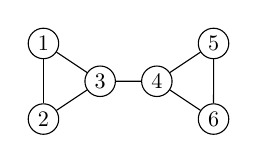
\begin{tikzpicture}[scale=0.6, every node/.style={scale=0.8,inner sep=.7mm}]
          \node [draw,circle] (1) at (0,1.6) {1};
          \node [draw,circle] (2) at (0,0) {2};
          \node [draw,circle] (3) at (1.2,.8) {3};
          \node [draw,circle] (4) at (2.4,.8) {4};
          \node [draw,circle] (5) at (3.6,1.6) {5};
          \node [draw,circle] (6) at (3.6,0) {6};
          \draw (1) -- (2);
          \draw (1) -- (3);
          \draw (2) -- (3);
          \draw (3) -- (4);
          \draw (4) -- (5);
          \draw (4) -- (6);
          \draw (5) -- (6);
        \end{tikzpicture}
        \label{fig:g1}
    }
    \quad\subfigure[][$G_2$] {
        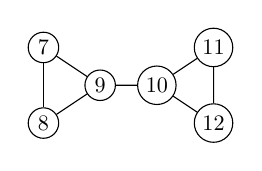
\begin{tikzpicture}[scale=0.6, every node/.style={scale=0.8,inner sep=.7mm}]
          \node [draw,circle] (1) at (0,1.6) {7};
          \node [draw,circle] (2) at (0,0) {8};
          \node [draw,circle] (3) at (1.2,.8) {9};
          \node [draw,circle] (4) at (2.4,.8) {10};
          \node [draw,circle] (5) at (3.6,1.6) {11};
          \node [draw,circle] (6) at (3.6,0) {12};
          \draw (1) -- (2);
          \draw (1) -- (3);
          \draw (2) -- (3);
          \draw (3) -- (4);
          \draw (4) -- (5);
          \draw (4) -- (6);
          \draw (5) -- (6);
        \end{tikzpicture}
        \label{fig:g2}
    }
    \quad\subfigure[][$G_3$] {
        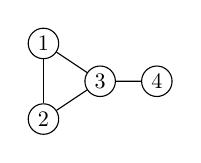
\begin{tikzpicture}[scale=0.6, every node/.style={scale=0.8,inner sep=.7mm}]
          \node [draw,circle] (1) at (0,1.6) {1};
          \node [draw,circle] (2) at (0,0) {2};
          \node [draw,circle] (3) at (1.2,.8) {3};
          \node [draw,circle] (4) at (2.4,.8) {4};
          \draw (1) -- (2);
          \draw (1) -- (3);
          \draw (2) -- (3);
          \draw (3) -- (4);
        \end{tikzpicture}
        \label{fig:g3}
    }
%    \quad\subfigure[][$G_4$] {
%        \begin{tikzpicture}[scale=0.6, every node/.style={scale=0.8,inner sep=.7mm}]
%          \node [draw,circle] (1) at (0,1.6) {1};
%          \node [draw,circle] (2) at (0,0) {2};
%          \node [draw,circle] (3) at (1.2,.8) {3};
%          \node [draw,circle] (4) at (2.4,1.6) {4};
%          \node [draw,circle] (5) at (2.4,0) {5};
%          \draw (1) -- (2);
%          \draw (1) -- (3);
%          \draw (2) -- (3);
%          \draw (3) -- (4);
%          \draw (3) -- (5);
%          \draw (4) -- (5);
%        \end{tikzpicture}
%        \label{fig:g4}
%    }
    \caption{Example graphs $G_1$ to $G_3$}
    \label{fig:intro-examples}
\end{figure}

A \emph{loop} is an edge from a vertex to itself. We assume throughout this
dissertation that graphs have no loops, except in clearly marked sections where
we discuss extensions of algorithms to graphs with loops.

The set of vertices adjacent to vertex $v \in V(G)$
is called the \emph{neighbourhood} of $v$, denoted $\N_G(v)$.
The \emph{degree} of a vertex is size of its neighbourhood.
We denote
by $\invN_G(v)$ the \emph{inverse neighbourhood} of $v$: the set
of the vertices other than $v$ itself that are not adjacent to $v$.
We omit the subscript $G$ where there is no ambiguity.
In \Cref{fig:g1}, for example, we have $\N(3) = \{1,2,4\}$ and
$\invN(3) = \{5,6\}$.

We say that graphs $G$ and $H$ are \emph{isomorphic} if they have the same
number of vertices and we can relabel the vertices of $G$ to produce graph $H$.
For example, graphs $G_1$ and $G_2$ in \Cref{fig:intro-examples} are
isomorphic.  Formally, an \emph{isomorphism} between graphs $G$ and $H$ is a
bijection $f:V(G)\rightarrow V(H)$, such that $E(H) = \{\{f(u), f(v)\} \mid \{u,
v\} \in E(G)\}$.  If such an $f$ exists, we say that $G$ and $H$ are
isomorphic.

The \emph{line graph} of a graph $G$ is a graph with a vertex for each element
of $E(G)$, such that two vertices are adjacent if and only if their corresponding edges
in $G$ share an endpoint.

An \emph{induced subgraph} of $G = (V, E)$ is a graph that has a subset $W \subseteq V$ as its
vertex set, and $\{\{u, v\} \in E \mid \{u, v\} \in W\}$ as its edge set; that
is, the subgraph includes all edges of $G$ whose endpoints both appear in
$W$.  We say that this subgraph is \emph{induced by} $W$.
Graph $G_3$ of \Cref{fig:intro-examples} is thus the subgraph
of $G_1$ induced by the set $\{1,2,3,4\}$.  We say that $G$ \emph{contains
$H$ as an induced subgraph} if $H$ is isomorphic to an induced subgraph of $G$.
A \emph{subgraph} (without the ``induced'' qualifier) is an induced subgraph
with zero or more edges deleted.

A \emph{common induced subgraph} of graphs $G$ and $H$ is an induced subgraph
of $G$ which is isomorphic to an induced subgraph of $H$. In
\Cref{fig:cis-example}, a common induced subgraph of the two graphs (which is
induced by $\{1,2,3,4\}$) is highlighted on the first graph, and its isomorphic
subgraph is highlighted on the second graph.  It is often convenient to summarise
a common induced subgraph and its associated isomorphism $f$ by the \emph{mapping}
$\{(v,f(v)) \mid v \in W\}$, where $W \subseteq V$ is the set of vertices that
induces the common subgraph.  In our example, $M = \{(1,6), (2,7), (3,8), (4,9)\}$.

\begin{figure}[h!]
\centering
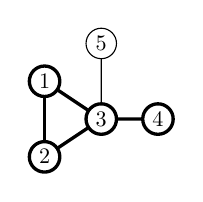
\begin{tikzpicture}[scale=0.6, every node/.style={scale=0.8,inner sep=.7mm}]
  \node [very thick,draw,circle] (1) at (0,1.6) {1};
  \node [very thick,draw,circle] (2) at (0,0) {2};
  \node [very thick,draw,circle] (3) at (1.2,.8) {3};
  \node [very thick,draw,circle] (4) at (2.4,.8) {4};
  \node [draw,circle] (5) at (1.2,2.4) {5};
  \draw [very thick] (1) -- (2);
  \draw [very thick] (1) -- (3);
  \draw [very thick] (2) -- (3);
  \draw [very thick] (3) -- (4);
  \draw (3) -- (5);
\end{tikzpicture}
\qquad
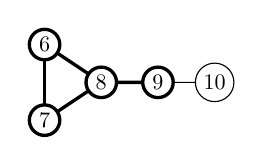
\begin{tikzpicture}[scale=0.6, every node/.style={scale=0.8,inner sep=.7mm}]
  \node [very thick,draw,circle] (1) at (0,1.6) {6};
  \node [very thick,draw,circle] (2) at (0,0) {7};
  \node [very thick,draw,circle] (3) at (1.2,.8) {8};
  \node [very thick,draw,circle] (4) at (2.4,.8) {9};
  \node [draw,circle] (5) at (3.6,.8) {10};
  \draw [very thick] (1) -- (2);
  \draw [very thick] (1) -- (3);
  \draw [very thick] (2) -- (3);
  \draw [very thick] (3) -- (4);
  \draw (4) -- (5);
\end{tikzpicture}
\caption{A pair of graphs with a maximum common induced subgraph highlighted}
\label{fig:cis-example}
\end{figure}

A \emph{maximum common induced subgraph (MCIS)} of $G$ and $H$ is a common
induced subgraph of $G$ and $H$ whose vertex set is as large as possible; the
common induced subgraph in \Cref{fig:cis-example} is an example of an MCIS.

A \emph{connected graph} is a graph $G=(V,E)$ such that for all $u,v \in V$,
we can reach vertex $v$ by beginning at vertex $u$ and traversing a sequence
of edges.

A \emph{clique} is a set of vertices that are mutually adjacent, and the
\emph{maximum clique problem} is, given a graph $G$, to find a clique in $G$
with as many vertices as possible.

A \emph{labelled graph} (or \emph{network}) is a triple $(G, f_v, f_e)$
where $G$ is a graph,
the \emph{vertex label function} $f_v$ is a function with domain $V(G)$,
and the \emph{edge label function} $f_e$ is a function with domain $E(G)$.
An isomorphism between labelled graphs is required to map each vertex of
$V$ to a vertex with the same label, and each edge to an edge with the same label.

A \emph{directed graph} is a pair $(V,A)$, where $V$ is the vertex set and $A$,
a set of ordered pairs of elements of $V$, is the arc set.  The definitions of
\emph{induced subgraph}, \emph{isomorphism} and \emph{maximum common induced
subgraph} for directed graphs are analogous to their counterparts for graphs.
\Cref{fig:directed-cis-example} shows two directed graphs with a common
induced subgraph highlighted.

\begin{figure}[h!]
\centering
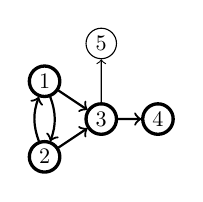
\begin{tikzpicture}[scale=0.6, every node/.style={scale=0.8,inner sep=.7mm}]
  \node [very thick,draw,circle] (1) at (0,1.6) {1};
  \node [very thick,draw,circle] (2) at (0,0) {2};
  \node [very thick,draw,circle] (3) at (1.2,.8) {3};
  \node [very thick,draw,circle] (4) at (2.4,.8) {4};
  \node [draw,circle] (5) at (1.2,2.4) {5};
  \draw [->,thick,bend left=20] (1) edge (2);
  \draw [->,thick,bend left=20] (2) edge (1);
  \draw [->,thick] (1) edge (3);
  \draw [->,thick] (2) edge (3);
  \draw [->,thick] (3) edge (4);
  \draw [->] (3) edge (5);
\end{tikzpicture}
\qquad
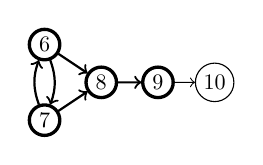
\begin{tikzpicture}[scale=0.6, every node/.style={scale=0.8,inner sep=.7mm}]
  \node [very thick,draw,circle] (1) at (0,1.6) {6};
  \node [very thick,draw,circle] (2) at (0,0) {7};
  \node [very thick,draw,circle] (3) at (1.2,.8) {8};
  \node [very thick,draw,circle] (4) at (2.4,.8) {9};
  \node [draw,circle] (5) at (3.6,.8) {10};
  \draw [->,thick,bend left=20] (1) edge (2);
  \draw [->,thick,bend left=20] (2) edge (1);
  \draw [->,thick] (1) edge (3);
  \draw [->,thick] (2) edge (3);
  \draw [->,thick] (3) edge (4);
  \draw [->] (4) edge (5);
\end{tikzpicture}
\caption{A pair of directed graphs with a maximum common induced subgraph highlighted}
\label{fig:directed-cis-example}
\end{figure}

For arc $(u,v)$, we say that $u$ is the source vertex and $v$ is target vertex; both
$u$ and $v$ are called endpoints.

The two most common representations of a graph in computer memory
are an \emph{adjacency matrix} and \emph{adjacency lists}.  For simplicity,
we assume that the vertices of a graph $G$ are numbered sequentially from
0 to $|V(G)| - 1$. The adjacency matrix representation is an $n \times n$
array $A$ of Boolean values, such that $A[v][w]$ is $\AlgVar{true}$ if and
only if $v$ and $w$ are adjacent.  The adjacency list representation
is a list of $n$ lists, with list $v$ containing the neighbours of vertex $v$.
The former representation allows us to test for the existence of an edge in constant
time.  The latter representation is space-efficient for sparse graphs
and allows us to iterate over the neighbourhood of a vertex in linear time.

There are numerous models for generating graphs randomly. Several are used
in this dissertation, and in general we will define these models at the point
of use.  A very common random graph model is the Erd\H{o}s-Rényi $G(n,p)$
model: for a given order $n \geq 0$ and edge probability $p$ ($0 \leq p \leq 1$),
the graph is generated by creating a set of $n$ nodes and adding an edge
between each pair of nodes with independent probability $p$.

\section{Computational Complexity}\label{sec:complexity}

This section gives a very brief, informal description of
\emph{\NP-hardness} and related concepts. A more complete introduction can be
found in the classic monograph of \citet{DBLP:books/fm/GareyJ79},
while \citet{moore2011nature} give a broader, and very entertaining,
treatment.

Consider the \textsc{Clique} problem: given a graph $G$ and a natural number $k$,
does $G$ contain a $k$-vertex clique?  If the answer is ``yes'', we can give a proof
of this fact by listing the $k$ vertices in this clique.  A sceptic may verify
in $k(k-1)/2$ steps that the $k$ vertices are indeed pairwise adjacent.  Any decision
problem---like \textsc{clique}---such that there is a proof of ``yes'' instances
that can be verified in polynomial time is said to be in the complexity class \NP.

Although we can verify a ``yes'' instance of \textsc{Clique} in polynomial
time, there is no known way to solve the problem in polynomial time.
Indeed \textsc{Clique} is, in an important sense, one of the hardest problems in \NP\
\citep{DBLP:conf/coco/Karp72}: every instance of a problem in \NP\ can be
transformed, or \emph{reduced}, to a \textsc{Clique} instance in polynomial
time, such that the original instance and the reduced instance give the same
answer.  Any problem in \NP\ that has this property is called \emph{\NP-complete}.

A problem $H$ is \emph{\NP-hard} if it is at least as hard as any problem in \NP;
that is, if any problem in \NP\ can be solved in polynomial time under the assumption
that we have an oracle that can solve $H$ in constant time.  We will see in the next
section that all three problems considered in this dissertation are \NP-hard.

TODO could lead on to a section on coping with complexity as relating to optimisation problems, i.e., exponential-time algorithms that "perform well in practice", e.g., based on branch and bound, integer and constraint programming, FPT algorithms,...
give theoretical bounds for current state of the art exponential-time algorithms for optimisation problems that you consider.

\section{Problems Covered by This Dissertation}\label{sec:problems}

This dissertation presents algorithms for the following three problems.
The first and third are optimisation problems; the second
is a decision problem.

\begin{itemize}
    \item \textbf{Maximum common induced subgraph (MCIS).} Find
a maximum common induced subgraph of two given graphs.  We have seen an example
in \Cref{fig:cis-example}: the two graphs have a maximum common induced subgraph
with four vertices.
    \item \textbf{Induced subgraph isomorphism (ISIP).} Given graphs $G$ (the ``pattern graph'')
    and $H$ (the ``target graph''),
determine whether $H$ contains $G$ as an induced subgraph;
if so, return the mapping corresponding to an isomorphism from $G$ to an
        induced subgraph of $H$.
    \Cref{fig:isip-examples} gives two examples of instances. The first is unsatisfiable;
        the solution $\{(1,a),(2,b), (3,d)\}$ for the second instance is shown.
    \item \textbf{Minimal induced universal graph.} Given a family of graphs $\calF$,
find a graph with as few vertices as possible that contains each member of $\calF$
as an induced subgraph.
    \Cref{fig:ind-univ-instance} shows an example instance: the family
        of graphs $\{C_3, C_4, C_5\}$.  
    \Cref{fig:ind-univ-solution} shows a corresponding solution with six vertices.
        This is shown three times, with an induced copy of each input graph
        highlighted.
\end{itemize}

\begin{figure}[htb]
    \centering
    \subfigure[][Unsatisfiable] {
        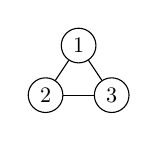
\begin{tikzpicture}[scale=0.7, every node/.style={scale=0.8,minimum width=.55cm,inner sep=.7mm}]
          \node [draw,circle] (1) at (.6,.9) {1};
          \node [draw,circle] (2) at (0,0) {2};
          \node [draw,circle] (3) at (1.2,0) {3};
          \draw (1) -- (2);
          \draw (1) -- (3);
          \draw (2) -- (3);
        \end{tikzpicture}\quad
        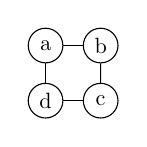
\begin{tikzpicture}[scale=0.7, every node/.style={scale=0.8,minimum width=.55cm,inner sep=.7mm}]
          \node [draw,circle] (a) at (0,1) {a};
          \node [draw,circle] (b) at (1,1) {b};
          \node [draw,circle] (c) at (1,0) {c};
          \node [draw,circle] (d) at (0,0) {d};
          \draw (a) -- (b);
          \draw (b) -- (c);
          \draw (c) -- (d);
          \draw (d) -- (a);
        \end{tikzpicture}
        \label{fig:si-unsat}
    }\qquad\qquad\subfigure[][Satisfiable] {
        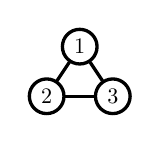
\begin{tikzpicture}[scale=0.7, every node/.style={scale=0.8,minimum width=.55cm,inner sep=.7mm}]
          \node [very thick,draw,circle] (1) at (.6,.9) {1};
          \node [very thick,draw,circle] (2) at (0,0) {2};
          \node [very thick,draw,circle] (3) at (1.2,0) {3};
          \draw [very thick] (1) -- (2);
          \draw [very thick] (1) -- (3);
          \draw [very thick] (2) -- (3);
        \end{tikzpicture}\quad
        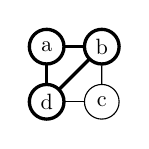
\begin{tikzpicture}[scale=0.7, every node/.style={scale=0.8,minimum width=.55cm,inner sep=.7mm}]
          \node [very thick,draw,circle] (a) at (0,1) {a};
          \node [very thick,draw,circle] (b) at (1,1) {b};
          \node [draw,circle] (c) at (1,0) {c};
          \node [very thick,draw,circle] (d) at (0,0) {d};
          \draw [very thick] (a) -- (b);
          \draw (b) -- (c);
          \draw (c) -- (d);
          \draw [very thick] (d) -- (a);
          \draw [very thick] (b) -- (d);
        \end{tikzpicture}
        \label{fig:si-sat}
    }
    \caption{Two instances of the induced subgraph isomorphism problem}
    \label{fig:isip-examples}
\end{figure}

\begin{figure}[htb]
    \centering
    \subfigure[][Instance] {
        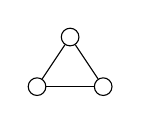
\begin{tikzpicture}[scale=0.7, every node/.style={scale=0.8,minimum width=.28cm,inner sep=.7mm}]
          \node [draw,circle] (1) at (.6,.9) {};
          \node [draw,circle] (2) at (0,0) {};
          \node [draw,circle] (3) at (1.2,0) {};
          \draw (1) -- (2);
          \draw (1) -- (3);
          \draw (2) -- (3);
        \end{tikzpicture}\quad
        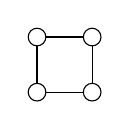
\begin{tikzpicture}[scale=0.7, every node/.style={scale=0.8,minimum width=.28cm,inner sep=.7mm}]
          \node [draw,circle] (a) at (0,1) {};
          \node [draw,circle] (b) at (1,1) {};
          \node [draw,circle] (c) at (1,0) {};
          \node [draw,circle] (d) at (0,0) {};
          \draw (a) -- (b);
          \draw (b) -- (c);
          \draw (c) -- (d);
          \draw (d) -- (a);
        \end{tikzpicture}\quad
        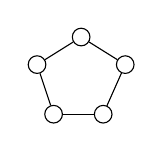
\begin{tikzpicture}[scale=0.7, every node/.style={scale=0.8,minimum width=.28cm,inner sep=.7mm}]
          \node [draw,circle] (a) at (-.2,.9) {};
          \node [draw,circle] (b) at (.6,1.4) {};
          \node [draw,circle] (c) at (1.4,.9) {};
          \node [draw,circle] (d) at (1,0) {};
          \node [draw,circle] (e) at (.1,0) {};
          \draw (a) -- (b);
          \draw (b) -- (c);
          \draw (c) -- (d);
          \draw (d) -- (e);
          \draw (e) -- (a);
        \end{tikzpicture}
        \label{fig:ind-univ-instance}
    }\qquad\qquad\subfigure[][A solution] {
        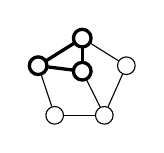
\begin{tikzpicture}[scale=0.7, every node/.style={scale=0.8,minimum width=.28cm,inner sep=.7mm}]
            \node [very thick,draw,circle] (a) at (-.2,.9) {};
          \node [very thick,draw,circle] (b) at (.6,1.4) {};
          \node [draw,circle] (c) at (1.4,.9) {};
          \node [draw,circle] (d) at (1,0) {};
          \node [draw,circle] (e) at (.1,0) {};
          \node [very thick,draw,circle] (f) at (.6,.8) {};
            \draw [very thick] (a) -- (b);
          \draw (b) -- (c);
          \draw (c) -- (d);
          \draw (d) -- (e);
          \draw (e) -- (a);
            \draw [very thick] (a) -- (f);
          \draw (f) -- (d);
            \draw [very thick] (f) -- (b);
        \end{tikzpicture}\quad
        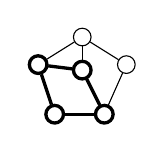
\begin{tikzpicture}[scale=0.7, every node/.style={scale=0.8,minimum width=.28cm,inner sep=.7mm}]
            \node [very thick,draw,circle] (a) at (-.2,.9) {};
          \node [draw,circle] (b) at (.6,1.4) {};
          \node [draw,circle] (c) at (1.4,.9) {};
          \node [very thick,draw,circle] (d) at (1,0) {};
          \node [very thick,draw,circle] (e) at (.1,0) {};
          \node [very thick,draw,circle] (f) at (.6,.8) {};
          \draw (a) -- (b);
          \draw (b) -- (c);
          \draw (c) -- (d);
            \draw [very thick] (d) -- (e);
            \draw [very thick] (e) -- (a);
            \draw [very thick] (a) -- (f);
            \draw [very thick] (f) -- (d);
          \draw (f) -- (b);
        \end{tikzpicture}\quad
        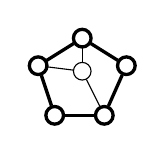
\begin{tikzpicture}[scale=0.7, every node/.style={scale=0.8,minimum width=.28cm,inner sep=.7mm}]
            \node [very thick,draw,circle] (a) at (-.2,.9) {};
          \node [very thick,draw,circle] (b) at (.6,1.4) {};
          \node [very thick,draw,circle] (c) at (1.4,.9) {};
          \node [very thick,draw,circle] (d) at (1,0) {};
          \node [very thick,draw,circle] (e) at (.1,0) {};
          \node [draw,circle] (f) at (.6,.8) {};
            \draw [very thick] (a) -- (b);
            \draw [very thick] (b) -- (c);
            \draw [very thick] (c) -- (d);
            \draw [very thick] (d) -- (e);
            \draw [very thick] (e) -- (a);
          \draw (a) -- (f);
          \draw (f) -- (d);
          \draw (f) -- (b);
        \end{tikzpicture}
        \label{fig:ind-univ-solution}
    }
    \caption{An instance of the minimal induced universal graph problem, and a solution}
    \label{fig:induced-universal-example}
\end{figure}

Each
of the three problems can be seen to be \NP-hard by a simple reduction from
\textsc{Clique}, which may be seen as follows.
Given graph $G$ and natural number $k$, we can determine whether $G$ contains a clique
of size $k$ by solving either of the first two problems with the complete graph $K_k$ as
the first graph and $G$ as the second graph, or by solving the third problem with the family
$\{K_k, G\}$ as the input.

All three problems remain \NP-hard if the input graphs are both forests
\citep{DBLP:books/fm/GareyJ79}, or are both series-parallel graphs
\citep{syslo1982induced}.

Each problem has a natural extension to labelled graphs
where we require the isomorphism to preserve labels on vertices and edges.
Likewise, each problem has a variant for directed graphs.
For the first two problems, this dissertation presents algorithms for both
labelled graphs and directed graphs; for the third problem we only consider
unlabelled, undirected graphs.

All three problems have natural enumeration counterparts:
to find all maximum common induced subgraphs, all induced subgraph isomorphisms,
and all minimal induced univeral graphs.  As we will see in the following
chapters, our solvers can be straightforwardly extended to handle
these enumeration versions.

\section{Related Problems}\label{sec:related-problems}

This section briefly introduces three problems that are closely related to
maximum common induced subgraph and induced subgraph isomorphism.

The \emph{graph isomorphism problem} is to determine whether two given graphs are
isomorphic. It can be viewed as a version the induced subgraph isomorphism
problem that returns ``no'' if the input graphs do not have the same number of
vertices.  It is unknown whether the problem is \NP-complete, and it is also
unknown whether it can be solved in polynomial time, although a
quasipolynomial-time algorithm has been proposed
\citep{DBLP:conf/stoc/Babai16}.  Most state of the art algorithms for graph
isomorphism, such as Nauty and Traces \citep{DBLP:journals/jsc/McKayP14}, solve the problem by computing a
canonical representation of each graph and comparing these representations.
This method has the advantage that the canonical
representations may then be re-used for comparisons with other graphs.
Considering only pairwise comparisons of graphs, a 2001 study found that the
induced subgraph isomorphism solver VF2 outperformed Nauty on several classes
of graphs \citep{foggia2001performance}.  While we do not consider graph
isomorphism further in this dissertation, it would be an interesting topic of
future work to test whether the current state of the art subgraph isomorphism
solvers outperform the best graph isomorphism solvers on some interesting
classes of graphs.

Induced subgraph isomorphism and maximum common induced subgraph each have a
non-induced counterpart. The \emph{subgraph monomorphism problem} is to
determine whether graph $G$ is isomorphic to a subgraph of graph $H$, without
the requirement that the subgraph be induced.  Some papers use the name
\emph{subgraph isomorphism} to refer to subgraph monomorphism
\citep{DBLP:conf/cp/McCreeshP15}, while others use the same name to refer to induced
subgraph isomorphism \citep{DBLP:journals/pami/CarlettiFSV18}.  To avoid
confusion, the ambiguous term ``subgraph isomorphism'' (without the ``induced''
qualifier) will not be used in the sequel.

The \emph{maximum common edge subgraph (MCES)} problem is to find a subgraph of
graph $G$ with as many edges (rather than vertices) as possible that is
isomorphic to a subgraph of graph $H$, again without requiring that the
subgraphs be induced.  There is a non-trivial but close connection between this
problem and MCIS: by a result due to \citet{whitney1932congruent}, we can find
the MCES two graphs by searching for an MCIS on their line graphs.  This
approach has a small complication: the triangle graph $K_3$ and the claw graph
$K_{1,3}$ (\cref{fig:k3-and-claw}) both have $K_3$ as their line graph, and we
must therefore check during search that no strongly connected component of $G$
that is a triangle (resp.\ claw) is mapped to a claw (resp.\ triangle) in $H$.

\begin{figure}[htb]
    \centering
    \begin{tikzpicture}[scale=.35, every node/.style={black,scale=0.7}]%{{{
    \node[draw, circle, fill=white, inner sep=1.4pt, font=\bfseries] (Na) at (1,  0)
    {\vphantom{0}};
    \node[draw, circle, fill=white, inner sep=1.4pt, font=\bfseries] (Nb) at (0, -2)
    {\vphantom{0}};
    \node[draw, circle, fill=white, inner sep=1.4pt, font=\bfseries] (Nc) at (2, -2)
    {\vphantom{0}};

    \draw [edge] (Na) -- (Nb);
    \draw [edge] (Nb) -- (Nc);
    \draw [edge] (Na) -- (Nc);

\end{tikzpicture}
\qquad
\begin{tikzpicture}[scale=.35, every node/.style={black,scale=0.7}]%{{{
    \node[draw, circle, fill=white, inner sep=1.4pt, font=\bfseries] (Na) at (-.2,  -.2)
    {\vphantom{0}};
    \node[draw, circle, fill=white, inner sep=1.4pt, font=\bfseries] (Nb) at (2.2, -.2)
    {\vphantom{0}};
    \node[draw, circle, fill=white, inner sep=1.4pt, font=\bfseries] (Nc) at (1, -1.5)
    {\vphantom{0}};
    \node[draw, circle, fill=white, inner sep=1.4pt, font=\bfseries] (Nd) at (1, -3)
    {\vphantom{0}};

    \draw [edge] (Na) -- (Nc);
    \draw [edge] (Nb) -- (Nc);
    \draw [edge] (Nc) -- (Nd);

\end{tikzpicture}

    \caption{The graphs $K_3$ and $K_{1,3}$.}
    \label{fig:k3-and-claw}
\end{figure}

Several algorithms for MCES, such as RASCAL
\citep{DBLP:journals/cj/RaymondGW02}, use this line graph method, as we will discuss further
in the next section.  \citet{DBLP:conf/mco/VismaraV08} describe how this technique
can be used on labelled graphs.

The present author's preliminary work on using the \McSplit\ algorithm
described in this thesis for MCES using line graphs shows promising results
\citep{trimble2018three}. This would be a useful direction for future work, but
it is not pursued further in this dissertation.

A generalisation that can be applied to any variant of the maximum common subgraph
problem is to find the maximum common subgraph of an arbitrary set of graphs,
rather than only of a pair of graph.  The MCES version of this problem has
been studied in the context of sets of molecules
\citep{DBLP:journals/jcheminf/DalkeH13}.

%The maximum clique problem is to find an induced subgraph of a graph $G$ with as
%many vertices as possible, such that the subgraph has all possible edges; that
%is ??. Maximum clique can be solved (although rather inefficiently in practice)
%using an MCIS algorithm, by finding the MCIS of $G$ and a complete graph with the
%same number of vertices as $G$.

\section{Constraint Programming}\label{sec:cp}

We now turn from problems to solution methods.  As discussed previously, each
problem studied in this dissertation is \NP-hard.  This section reviews
\emph{constraint programming}, a very general framework for modelling and
solving \NP-hard problems which is the basis of many existing solvers for
maximum common subgraph and induced subgraph isomorphism, and which has close
connections to the \McSplit\ algorithms that we will introduce.

A \emph{constraint satisfaction problem (CSP)} is a problem of finding a value
for each of a finite set of variables with finite domains, subject to a set of constraints.
This framework is extremely broad, and has applications in fields
including logistics, scheduling, bioinformatics, and discrete mathematics.
The field of \emph{constraint programming (CP)} is concerned with modelling
and solving CSPs and related problems.

Many algorithms
for MCIS and induced subgraph isomorphism model the problems as CSPs.
Moreover, the \McSplit\ family of algorithms that will be introduced in the next three chapters
are closely related to a constraint programming approach.
This section gives a brief introduction to constraint programming;
a detailed treatment can be found in the \emph{Handbook of Constraint
Programming} \citep{DBLP:reference/fai/2}.

Formally, a CSP is a triple $\langle X, D, C\rangle$, where

\begin{itemize}
\item $X$ is a tuple of \emph{variables} $X = \langle x_1, x_2, \dots, x_n \rangle$,
\item $D$ is a corresponding tuple of finite \emph{domains} $D = \langle D_1, D_2, \dots, D_n\rangle$
  such that each $x_i$ must take a value in $D_i$,
\item $C$ is a set of constraints, each of which acts on a subset of $X$ and restricts
  the values that may be taken simultaneously by those variables.
\end{itemize}

A solution to a CSP is an assignment of domain values to each variable in $X$
satisfying the constraints $C$.

Broadly, algorithms for solving CSPs can be classed as \emph{complete} (guaranteed to find a solution
if one exists)
or \emph{incomplete}. The former category is the focus of this dissertation.
All of the constraint programming approaches to MCIS and induced
subgraph isomorphism use some form of backtracking search, and therefore that will
be the focus of this section.

To illustrate the process of solving a CSP by backtracking, we use a canonical
introductory problem, $n$-queens. For our example, we will consider the case
$n=4$. The problem is to place four queens on a $4 \times 4$ chessboard such
that no two queens are in the same row, column, or diagonal.

The first step is to model the problem as a CSP. Many models have been proposed
for the $n$-queens problem \citep{DBLP:reference/fai/Smith06}; we will use a
simple model with one variable per row ($x_1$ to $x_4$) and four values, $\{a, b, c, d\}$, for
the four columns.  There are two types of constraint. First, there is a single
\emph{allDifferent} constraint to ensure that the four variables take different
values (and thus the queens are in different columns). Second, there is a
constraint for each of ten diagonals
ensuring that at most one queen is placed on that diagonal.
(The one-queen-per-row requirement is met without further constraints,
since each variable must take exactly one value.)

\Cref{fig:FourQueens} shows a search tree for this problem.
This tree is traversed in depth-first order, and is not explicitly
stored.
At node \treenode{A},
no assignments of values to variables have been made. At node \treenode{B}, a first
tentative assignment has been made: $x_1=a$. A key part of most backtracking CP
solvers is the interleaving of search (trying possible values for a variable
in turn) with \emph{constraint propagation} (deleting values that can be
determined not to appear in any solution that extends the current set of
assignments). For our example, we will use the simplest form of propagation:
\emph{forward checking}. This removes from the domains of the unassigned variables
every value that conflicts with some existing assignment. The $\times$ symbol
in a square in the figure indicates that a value has been removed from a domain.

At node \treenode{C}, the assignment $x_2=c$ has been made. After forward checking, no
values are left in $D_3$; thus there is no solution with $x_1=a$ and $x_2=c$.
The algorithm backtracks and tries $x_2=d$
(node \treenode{D}). This process of search, forward checking, and backtracking when
a domain becomes empty is continued (nodes \treenode{E} to \treenode{I}) until reaching the solution
shown in node \treenode{I}.

\newsavebox{\FourQueensBoxA}
\newsavebox{\FourQueensBoxB}
\newsavebox{\FourQueensBoxC}
\newsavebox{\FourQueensBoxD}
\newsavebox{\FourQueensBoxE}
\newsavebox{\FourQueensBoxF}
\newsavebox{\FourQueensBoxG}
\newsavebox{\FourQueensBoxH}
\newsavebox{\FourQueensBoxI}
\sbox{\FourQueensBoxA}{\FourQueens{A}{0.5/0.5/,1.5/0.5/,2.5/0.5/,3.5/0.5/,0.5/1.5/,1.5/1.5/,2.5/1.5/,3.5/1.5/,0.5/2.5/,1.5/2.5/,2.5/2.5/,3.5/2.5/,0.5/3.5/,1.5/3.5/,2.5/3.5/,3.5/3.5/}}
\sbox{\FourQueensBoxB}{\FourQueens{B}{0.5/0.5/\symqueen,1.5/0.5/$\times$,2.5/0.5/$\times$,3.5/0.5/$\times$,0.5/1.5/$\times$,1.5/1.5/$\times$,2.5/1.5/,3.5/1.5/,0.5/2.5/$\times$,1.5/2.5/,2.5/2.5/$\times$,3.5/2.5/,0.5/3.5/$\times$,1.5/3.5/,2.5/3.5/,3.5/3.5/$\times$}}
\sbox{\FourQueensBoxC}{\FourQueens{C}{0.5/0.5/\symqueen,1.5/0.5/$\times$,2.5/0.5/$\times$,3.5/0.5/$\times$,0.5/1.5/$\times$,1.5/1.5/$\times$,2.5/1.5/\symqueen,3.5/1.5/$\times$,0.5/2.5/$\times$,1.5/2.5/$\times$,2.5/2.5/$\times$,3.5/2.5/$\times$,0.5/3.5/$\times$,1.5/3.5/,2.5/3.5/$\times$,3.5/3.5/$\times$}}
\sbox{\FourQueensBoxD}{\FourQueens{D}{0.5/0.5/\symqueen,1.5/0.5/$\times$,2.5/0.5/$\times$,3.5/0.5/$\times$,0.5/1.5/$\times$,1.5/1.5/$\times$,2.5/1.5/$\times$,3.5/1.5/\symqueen,0.5/2.5/$\times$,1.5/2.5/,2.5/2.5/$\times$,3.5/2.5/$\times$,0.5/3.5/$\times$,1.5/3.5/$\times$,2.5/3.5/,3.5/3.5/$\times$}}
\sbox{\FourQueensBoxE}{\FourQueens{E}{0.5/0.5/\symqueen,1.5/0.5/$\times$,2.5/0.5/$\times$,3.5/0.5/$\times$,0.5/1.5/$\times$,1.5/1.5/$\times$,2.5/1.5/$\times$,3.5/1.5/\symqueen,0.5/2.5/$\times$,1.5/2.5/$\times$,2.5/2.5/\symqueen,3.5/2.5/$\times$,0.5/3.5/$\times$,1.5/3.5/$\times$,2.5/3.5/$\times$,3.5/3.5/$\times$}}
\sbox{\FourQueensBoxF}{\FourQueens{F}{0.5/0.5/$\times$,1.5/0.5/\symqueen,2.5/0.5/$\times$,3.5/0.5/$\times$,0.5/1.5/$\times$,1.5/1.5/$\times$,2.5/1.5/$\times$,3.5/1.5/,0.5/2.5/,1.5/2.5/$\times$,2.5/2.5/,3.5/2.5/$\times$,0.5/3.5/,1.5/3.5/$\times$,2.5/3.5/,3.5/3.5/}}
\sbox{\FourQueensBoxG}{\FourQueens{G}{0.5/0.5/$\times$,1.5/0.5/\symqueen,2.5/0.5/$\times$,3.5/0.5/$\times$,0.5/1.5/$\times$,1.5/1.5/$\times$,2.5/1.5/$\times$,3.5/1.5/\symqueen,0.5/2.5/,1.5/2.5/$\times$,2.5/2.5/$\times$,3.5/2.5/$\times$,0.5/3.5/,1.5/3.5/$\times$,2.5/3.5/,3.5/3.5/$\times$}}
\sbox{\FourQueensBoxH}{\FourQueens{H}{0.5/0.5/$\times$,1.5/0.5/\symqueen,2.5/0.5/$\times$,3.5/0.5/$\times$,0.5/1.5/$\times$,1.5/1.5/$\times$,2.5/1.5/$\times$,3.5/1.5/\symqueen,0.5/2.5/\symqueen,1.5/2.5/$\times$,2.5/2.5/$\times$,3.5/2.5/$\times$,0.5/3.5/$\times$,1.5/3.5/$\times$,2.5/3.5/,3.5/3.5/$\times$}}
\sbox{\FourQueensBoxI}{\FourQueens{I}{0.5/0.5/$\times$,1.5/0.5/\symqueen,2.5/0.5/$\times$,3.5/0.5/$\times$,0.5/1.5/$\times$,1.5/1.5/$\times$,2.5/1.5/$\times$,3.5/1.5/\symqueen,0.5/2.5/\symqueen,1.5/2.5/$\times$,2.5/2.5/$\times$,3.5/2.5/$\times$,0.5/3.5/$\times$,1.5/3.5/$\times$,2.5/3.5/\symqueen,3.5/3.5/$\times$}}

\begin{figure}[h!]
\centering
\begin{forest}
[\usebox{\FourQueensBoxA}
  [\usebox{\FourQueensBoxB}
    [\usebox{\FourQueensBoxC}]
    [\usebox{\FourQueensBoxD} [\usebox{\FourQueensBoxE}]]
  ]
  [\usebox{\FourQueensBoxF}
    [\usebox{\FourQueensBoxG}
      [\usebox{\FourQueensBoxH}
        [\usebox{\FourQueensBoxI}]
      ]
    ]
  ]
]
\end{forest}
\caption{The search tree of a backtracking CP algorithm for the 4-queens problem.}
\label{fig:FourQueens}
\end{figure}

For many problems, more costly propagation algorithms can remove more values
from domains than forward checking, achieving stronger \emph{levels of consistency}
(a level of consistency is a guarantee that a value will be removed from a domain
if some condition is met). It is common for constraint programming solvers to
maintain \emph{arc consistency}, guaranteeing that no value will remain in a domain
if there is some constraint involving two variables that cannot be satisfied if that
value is taken. \emph{Generalised arc consistency} extends this to constraints
involving arbitrarily many variables.
The canonical example is R{\'{e}}gin's polynomial-time filtering algorithm for the
allDifferent constraint, which uses a matching algorithm \citep{DBLP:conf/aaai/Regin94}.

The forward-checking search described above can be modified in numerous ways, many
of which are significant research topics in their own right. To give four examples:

\begin{itemize}
    \item We could break symmetries (informally, to ignore parts of the search tree
        that are equivalent to ones already visited) \citep{DBLP:reference/fai/GentPP06}.
	In the 4-queens example,
        we can disregard $x_1=c$ and $x_1=d$, since any solution with these assignments
        is the same as a solution with $x_1=b$ and $x_1=d$ after reflecting the chessboard
        horizontally.
    \item We could use a \emph{variable ordering heuristic} to choose which variable
    	to branch on at each search node, and a \emph{value ordering heuristic} to choose
	the order in which the child nodes of a search node are visited.
	For example, a very common variable ordering heuristic is to choose the variable
	with fewest remaining values \citep{golomb1965backtrack}.
    \item We could learn new constraints during search that do not affect the solution,
    	and use these to prune the search tree \citep{DBLP:conf/aaai/KatsirelosB05}.
    \item We could traverse the search tree in an order other than depth-first search
    	to quickly explore diverse regions of the search space.  An early
	example is limited discrepancy search \citep{DBLP:conf/ijcai/HarveyG95};
	another strategy is to combine the learning of constraints with periodic
	restarts of the backtracking search and randomised variable- and value-ordering
	heuristics
	\citep{DBLP:journals/jsat/LecoutreSTV07,DBLP:conf/cpaior/ArchibaldDHMP019}.
\end{itemize}

\newsavebox{\MCSDomainsBoxA}
\newsavebox{\MCSDomainsBoxB}
\newsavebox{\MCSDomainsBoxC}
\newsavebox{\MCSDomainsBoxD}
\sbox{\MCSDomainsBoxA}{\MCSDomains{A}{0.5/4.5/,1.5/4.5/,2.5/4.5/,3.5/4.5/,4.5/4.5/,5.5/4.5/,0.5/3.5/,1.5/3.5/,2.5/3.5/,3.5/3.5/,4.5/3.5/,5.5/3.5/,0.5/2.5/,1.5/2.5/,2.5/2.5/,3.5/2.5/,4.5/2.5/,5.5/2.5/,0.5/1.5/,1.5/1.5/,2.5/1.5/,3.5/1.5/,4.5/1.5/,5.5/1.5/,0.5/0.5/,1.5/0.5/,2.5/0.5/,3.5/0.5/,4.5/0.5/,5.5/0.5/}}
\sbox{\MCSDomainsBoxB}{\MCSDomains{B}{0.5/4.5/M,1.5/4.5/$\times$,2.5/4.5/$\times$,3.5/4.5/$\times$,4.5/4.5/$\times$,5.5/4.5/$\times$,0.5/3.5/$\times$,1.5/3.5/$\times$,2.5/3.5/$\times$,3.5/3.5/,4.5/3.5/$\times$,5.5/3.5/,0.5/2.5/$\times$,1.5/2.5/$\times$,2.5/2.5/$\times$,3.5/2.5/,4.5/2.5/$\times$,5.5/2.5/,0.5/1.5/$\times$,1.5/1.5/,2.5/1.5/,3.5/1.5/$\times$,4.5/1.5/,5.5/1.5/$\times$,0.5/0.5/$\times$,1.5/0.5/,2.5/0.5/,3.5/0.5/$\times$,4.5/0.5/,5.5/0.5/$\times$}}
\sbox{\MCSDomainsBoxC}{\MCSDomains{C}{0.5/4.5/M,1.5/4.5/$\times$,2.5/4.5/$\times$,3.5/4.5/$\times$,4.5/4.5/$\times$,5.5/4.5/$\times$,0.5/3.5/$\times$,1.5/3.5/$\times$,2.5/3.5/$\times$,3.5/3.5/M,4.5/3.5/$\times$,5.5/3.5/$\times$,0.5/2.5/$\times$,1.5/2.5/$\times$,2.5/2.5/$\times$,3.5/2.5/$\times$,4.5/2.5/$\times$,5.5/2.5/,0.5/1.5/$\times$,1.5/1.5/$\times$,2.5/1.5/$\times$,3.5/1.5/$\times$,4.5/1.5/,5.5/1.5/$\times$,0.5/0.5/$\times$,1.5/0.5/,2.5/0.5/,3.5/0.5/$\times$,4.5/0.5/$\times$,5.5/0.5/$\times$}}
\sbox{\MCSDomainsBoxD}{\MCSDomains{D}{0.5/4.5/M,1.5/4.5/$\times$,2.5/4.5/$\times$,3.5/4.5/$\times$,4.5/4.5/$\times$,5.5/4.5/$\times$,0.5/3.5/$\times$,1.5/3.5/$\times$,2.5/3.5/$\times$,3.5/3.5/M,4.5/3.5/$\times$,5.5/3.5/$\times$,0.5/2.5/$\times$,1.5/2.5/$\times$,2.5/2.5/$\times$,3.5/2.5/$\times$,4.5/2.5/$\times$,5.5/2.5/M,0.5/1.5/$\times$,1.5/1.5/$\times$,2.5/1.5/$\times$,3.5/1.5/$\times$,4.5/1.5/$\times$,5.5/1.5/$\times$,0.5/0.5/$\times$,1.5/0.5/,2.5/0.5/,3.5/0.5/$\times$,4.5/0.5/$\times$,5.5/0.5/$\times$}}

\subsection{A Simple CP Model for Induced Subgraph Isomorphism}
\label{subsec:cp-model-isip}

We now introduce a simple CSP formulation for induced subgraph isomorphism
based on \citet{ullmann1976algorithm}.
Let $G$ and $H$ be the pattern and target graphs.  We have a variable
$x_v$ for each $v \in V(G)$. The domain of each variable is $V(H)$, representing
the vertices in $H$ to which each vertex in $G$ may be mapped.
We have an allDifferent($\{x_v \mid v \in V(G)\}$) constraint to ensure that
all of the vertices in the pattern graph are mapped to different vertices
in the target graph.  Finally, we have two sets of constraints to ensure that edges in the pattern graph
are mapped to edges in the target graph and non-edges are mapped to non-edges:

\begin{itemize}
    \item For all distinct $v, w \in V(G)$ such that $v \in N_G(w)$, we have 
$x_v \in N_H(x_w)$.
\item For all distinct $v, w \in V(G)$ such that $v \not\in N_G(w)$, we have 
$x_v \not\in N_H(x_w)$.
\end{itemize}

\Cref{fig:SipDomains} shows one branch of the search tree for this CSP,
using graphs $G$ and $H$ in \Cref{fig:intro-G-H}.  Again, we show
each domain as a row, with the symbol $\times$ indicating that a value
has been removed. The letter $M$ indicates an assignment.

At node \treenode{B} of the search tree, variable $x_1$ has been assigned the value $a$,
corresponding to vertex 1 of graph $G$ being mapped to vertex $a$ of graph $H$. The
allDifferent propagator removes $a$ from the remaining four domains.
Values $b$ to $e$ are divided between those four domains---variables
$x_4$ and $x_5$ keep the vertices adjacent to $a$ in graph $H$ because vertices 4 and
5 are adjacent to vertex 1 in graph $G$.  At this and all of the other search
nodes, any two variables have either identical domains or disjoint domains;
in the next chapter this property will be exploited to develop what is essentially a compressed
domain store in the \McSplit\ algorithm.

\begin{figure}[h!]
\centering
    \scalebox{.8}{
        \tikz {
            \graph [nodes={draw, circle, minimum width=.55cm, inner sep=1pt}, circular placement, radius=0.95cm,
                    clockwise=5] {
                        1,2,3,4,5;
                1--4; 1--5; 2--3; 2--5; 3--5;
            };
        }
        \qquad\qquad
        \tikz {
            \graph [nodes={draw, circle, minimum width=.55cm, inner sep=1pt}, circular placement, radius=0.95cm,
                    clockwise=6, phase=60] {
                        a,b,c,d,e,f;
                a--b; a--c; a--e; b--d; b--f; c--d; c--e; c--f; d--f; e--f;
            };
        }
    }
\caption{Example graphs $G$ and $H$}
\label{fig:intro-G-H}
\end{figure}

\begin{figure}[h!]
\centering
\begin{forest}
[\usebox{\MCSDomainsBoxA}
  [\usebox{\MCSDomainsBoxB}
    [\usebox{\MCSDomainsBoxC}
      [\usebox{\MCSDomainsBoxD}]%[$\dots$]
    ]
    %[$\dots$]
  ]
  %[$\dots$]
]
\end{forest}
\caption{A branch of the search tree using forward checking for a simple constraint programming model
	of induced subgraph isomorphism}
\label{fig:SipDomains}
\end{figure}

\subsection{Constraint Optimisation Problems}

The previous subsection described constraint satisfaction problems, which are a
class of decision problem. We now turn to \emph{constraint optimisation
problems (COP)}, in which we must optimise some objective function.  The term
``constraint optimisation problem'' has multiple definitions in the literature;
we will define a COP simply as a modified CSP in which the goal is to minimise
or maximise a specific variable rather than determine satisfiability.

Branch and bound \citep{land2010automatic} is a general technique for solving
optimisation problems by backtracking search. We will describe branch and bound
in the context of maximisation problems.  
During search, we maintain an incumbent---the best solution found so far. Each
time a solution $S$ whose objective value is larger than the incumbent is found,
the incumbent’s value is updated to $S$. At each search node we calculate an
upper bound on the best objective value that can be obtained by extending the
current partial solution. If this upper bound is not greater than the
incumbent’s objective value, we know that exploring the subtree below the
current search node cannot possibly increase the incumbent, and it is therefore
safe to backtrack.

An alternative to branch and bound is to solve the maximisation problem by a
sequence of decision problems.  A simple way to do this, assuming that the
variable to be optimised is an integer variable, is to start with an optimistic
target and decrement this each time our search fails.  Beginning at a known
upper bound $b$ for the optimal objective value, we use search to answer the
question “does a solution with objective value $b$ exist?” If the answer is
“yes”, the algorithm terminates. Otherwise, a solution with objective value
$b-1$ is sought, then $b-2$, and so on until a solution is found.

In the next chapter, we compare these two techniques empirically for
the \McSplit\ algorithm.

\section{Algorithms for Induced Subgraph Isomorphism}\label{sec:si-algorithms}

This section reviews the two main lineages of practical algorithms
for induced subgraph isomorphism.  \Cref{subsec:cp-sip} reviews algorithms
based on constraint programming.  Many CP algorithms for induced subgraph
isomorphism are based on algorithms for subgraph monomorphism, and this
subsection therefore touches on the latter problem.  \Cref{subsec:pr-sip}
reviews algorithms from the pattern recognition community. These are in general
simple backtracking algorithms without the domain store used by constraint
programming algorithms.  Finally, \Cref{subsec:other-approaches-sip} reviews
other approaches.

\subsection{Algorithms Based on Constraint Programming}\label{subsec:cp-sip}

The algorithm of \citet{ullmann1976algorithm} solves only the subgraph
monomorphism problem.  The constraint programming model it uses is essentially
the one described in \Cref{subsec:cp-model-isip}, with the non-neighbour
constraints removed.  (We could trivially add these constraints to Ullmann's
algorithm to solve the induced problem.) The algorithm uses forward checking
for the allDifferent constraint and maintains arc consistency on the adjacency
constraints.
Bitsets---Boolean arrays
packed into arrays of larger words---are used to represent domains and rows of each
adjacency matrix, allowing very fast updates to domains, particularly
if the pattern and target graphs are dense.

\citet{DBLP:journals/isci/McGregor79} introduces a modified version of
Ullmann's algorithm.  McGregor finds experimentally that the cost of
maintaining arc consistency throughout search outweighs the benefit; as a
compromise, McGregor enforces arc consistency only after assigning the first
pattern-graph vertex, and uses forward checking at deeper levels of the search
tree.
% McGregor uses a static variable ordering heuristic in which vertices
% with most constraints involving previously-instantiated vertices are selected
% first.

The subsequent trend has been largely in the direction of more sophisticated
filtering at each search node.  This trend begins with the RESYN system
\citep{vism92,regin1995developpement}, whose filtering algorithm achieves
generalised arc consistency on the allDifferent constraint.

% The ILF(k) algorithm \citep{DBLP:journals/constraints/ZampelliDS10} introduces a
% filtering algorithm based on assigning during search a label to each vertex of
% the pattern graph and the target graph, with a partial ordering
% over the labels such that $v \in \V(G)$ may be assigned to $w \in V(H)$ if and
% only if $\mathit{label}(v) \preccurlyeq \mathit{label}(w)$.  Labels are
% iteratively extended to include information about the labels of neighbouring
% vertices.  Although this algorithm is described and implemented only for
% subgraph monomorphism, it appears that it could be
% extended to solve induced subgraph isomorphism.  (Like ILF(k), the \McSplit\ family of
% algorithms described in this dissertation may be viewed as assigning a label to
% each vertex and requiring that only vertices with compatible labels be assigned
% to one another. Unlike ILF(k), however, \McSplit\ requires labels to be equal.
% While this restricts the information that the \McSplit\ labels may
% contain, it results in very fast and simple constraint propagation in the
% \McSplit\ algorithm.)

\citet{DBLP:journals/ai/Solnon10} proposes an algorithm for LAD (local all
different) filtering, which propagates the following constraint: if $v \in
V(G)$ is mapped to $w \in V(H)$, then the neighbours of $v$ in $G$ must all be
mapped to different values, and these values must all belong to the set
$N_H(w)$.  This strengthens the filtering of the nRF+ algorithm
\citep{DBLP:journals/mscs/LarrosaV02}, and can be performed in $O(|V(G)| \cdot
|V(H)| \cdot \Delta_G^2 \cdot \Delta_H^2)$ time, where $\Delta_G$ and
$\Delta_H$ are the maximum degrees of $G$ and $H$.

The SND algorithm \citep{DBLP:conf/cp/AudemardLMGP14} extends LAD by counting
the number of length-$k$ paths between pairs of vertices for small values of
$k$, and enforcing within a LAD-style constraint that a pair of pattern
vertices connected by $p$ paths of length $k$ may not be mapped to a pair of
target vertices connected by fewer than $p$ paths of length $k$.  PathLAD
\citep{DBLP:conf/lion/KotthoffMS16} incorporates a subset of the SND filtering
into the LAD algorithm.

The Glasgow Subgraph Solver
\citep{DBLP:conf/cp/McCreeshP15,DBLP:conf/gg/McCreeshP020} (henceforth Glasgow)
reverses this trend towards stronger---and typically also slower---inference
at each search node.  The
algorithm aims to achieve most of the domain filtering of LAD and SND with much
less effort per search node.
The Glasgow algorithm introduces
\emph{supplemental graphs}---graphs that encode the number of paths
of a given length between pairs of vertices---which provide additional filtering
very cheaply.
%Unfortunately we cannot use the same technique in \McSplit-SI because
%it breaks the invariant, required by \McSplit-SI's data structure, that any two
%domains are either equal or disjoint.
Rather than achieving generalised arc consistency on the allDifferent
constraint, Glasgow uses a new ``counting'' allDifferent propagator which runs
very fast without giving any consistency guarantee.
Like Ullmann's algorithm, Glasgow uses bitsets to represent domains and rows
of adjacency matrices.
Glasgow was the fastest solver for hard induced
subgraph isomorphism instances in a recent experimental evaluation by
\citet{DBLP:conf/gbrpr/Solnon19}.

\paragraph*{Symmetry breaking}
\citet{zampelli2007symmetry} and \citet{DBLP:phd/basesearch/Zampelli08}
show that the variable and value symmetries
in the subgraph isomorphism problem can be completely broken using
the automorphism groups of the pattern and target graph graphs.
Moreover, the authors show how to break local symmetries that emerge
during search.
A solver with symmetry breaking was shown to be able to solve more instances
than the same solver without symmetry breaking. 
Techniques based on those of \citeauthor{zampelli2007symmetry} 
could be applied to any subgraph isomorphism solver based on constraint programming,
and the use of such techniques is understudied; neither \McSplit-SI nor any of
the state-of-the-art algorithms to which we compare it in our experiments
uses symmetry
breaking.\footnote{Recent versions of the Glasgow Subgraph Solver
have a symmetry breaking option for the pattern graph which is described as ``very experimental''.
We do not use this in our experiments.}  This would be a fruitful area for future
work.

\subsection{Pattern Recognition Algorithms}\label{subsec:pr-sip}

Algorithms for induced subgraph isomorphism from the pattern recognition (PR) community
take a lightweight approach---they do not store domains and perform
minimal work at each search node, resulting in algorithms with very low memory
requirements that can visit many search nodes per second, but often have to
visit many more search nodes in total than CP algorithms.

Like the CP solvers, the VF3 \citep{DBLP:journals/pami/CarlettiFSV18} and RI
\citep{DBLP:journals/bmcbi/BonniciGPSF13,DBLP:journals/tcbb/BonniciG17}
solvers explore a search tree, adding one pair of vertices to the mapping at each
search node.  However, the data structures maintained by these algorithms are
much more lightweight than those of any CP solver.  VF3 does not maintain
a domain for each vertex in the pattern graph; it simply store a partition
of the vertex set of each graph into three sets: ($A$) vertices that have been
mapped already, ($B$) unmapped vertices that are adjacent to at least one mapped vertex, and
($C$) all other unmapped vertices.
If the $B$ (resp.\ $C$) set of the target graph is smaller than the $B$ (resp.\ $C$)
set of the pattern graph, the algorithm can backtrack.
%This data structure can be updated with the same
%time complexity as the partitioning step of \McSplit-SI (and with a slightly
%smaller constant factor given the simplicity of the data structure).  
%However, its ability to prune the search tree is worse than that of \McSplit-SI
%since the $B$ sets are a union of the label classes in \McSplit-SI, and it
%leaves unavailable the smallest-domain-first heuristic used by \McSplit-SI.
RI is simpler still; it does not distinguish between sets $B$ and $C$.

RI-DS \citep{DBLP:journals/bmcbi/BonniciGPSF13} is a version of RI that
stores a domain for each vertex of $G$. These domains are filtered before search,
but the algorithm does not perform additional filtering during search.  Therefore,
the algorithm is more akin to the backtracking VF3 and RI solvers than to a
constraint programming solver.

\subsection{Other Approaches}\label{subsec:other-approaches-sip}

\citeauthor{sussenguth1965graph}'s (\citeyear{sussenguth1965graph})
backtracking algorithm for induced subgraph
isomorphism pre-dates the field of constraint programming but shares the
principle of interleaving search and propagation.  The algorithm uses
a list of rules to generate
pairs $\langle S_G, S_H \rangle$ such that $S_G \subseteq V(G)$, $S_H \subseteq
V(H)$, and each vertex in $S_G$ may only be mapped to vertices in $S_H$.
For example, pattern-graph vertices of degree 3 may only be mapped to
target-graph vertices of degree at least 3.
%Other properties used to
%generate pairs of sets include vertex labels and the size of the smallest cycle
%containing a vertex.
Further pairs of sets are generated based on adjacency to
members of these sets $S_G$ and $S_H$.
The search tree of Sussenguth's algorithm is incomparable to that of
other CP algorithms, and unfortunately an implementation of Sussenguth's
algorithm is not readily available.
(To preview the family of algorithms
presented in this dissertation, the \McSplit\ algorithm shares with
Sussenguth's algorithm the approach of storing pairs of sets $\langle S_G, S_H
\rangle$ representing vertices that may be mapped to one another. However,
\McSplit\ uses a very different data structure to store these sets, taking
advantage of the fact that the sets used by \McSplit\ are guaranteed to be
disjoint.)

\citet{DBLP:conf/RelMiCS/CortadellaV00} represent an instance of the subgraph
isomorphism problem as a binary decision diagram (BDD), and solve this BDD
in order to find all solutions to the subgraph isomorphism problem.  A limitation
is that for large
pattern graphs, the size of the BDDs quickly becomes unmanageable; the experiments
in the paper only consider pattern graphs with 10 or fewer vertices.

\paragraph*{Filter/verify} Some graph database systems use an indexing
technique to compute information about each target graph in a database, in the
hope that this can be used to quickly prove unsatisfiability for some pattern
graphs.  We do not consider this technique further because it not intended for
the one-shot problem of testing whether a given graph contains another graph as
in induced subgraph.  Moreover, it is unclear whether the filter/verify
technique provides any additional benefit over state of the art subgraph
isomorphism solvers; see \citet{DBLP:journals/jair/McCreeshPST18} for a
sceptical review.

% \paragraph*{SubGlw}
% The SubGlw solver \citep{DBLP:journals/access/AnsariJA21},
% which solves an incomplete enumeration problem: the problem of
% generating up to $k$ subgraph embeddings within a given time limit, for a given
% parameter $k$. To do this efficiently, the solver chooses a promising
% subgraph $S$ of the target graph, and runs the Glasgow Subgraph Solver in enumeration
% mode with pattern graph $G$ and target graph $S$. This avoids the overhead of
% building up the Glasgow solver's supplemental graph data structures for a large
% graph.  Since SubGlw is a small wrapper around an existing solver, and because
% it solves an incomplete enumeration problem that is not considered further
% in this thesis, we do not include it in our experimental evaluation.

\section{Algorithms for Maximum Common Induced Subgraph}\label{sec:mcs-algorithms}

%\textbf{TODO see \citet{DBLP:journals/jcamd/RaymondW02a} for a helpful lit review.
%Also Duesbury Holliday and Willett review}

Exact algorithms for the maximum common induced subgraph problem may be divided
into three broad categories: algorithms that solve the maximum clique problem
on a derived graph called the association graph, algorithms based on constraint
programming, and algorithms that enumerate subgraphs of graph $G$ and use a
subgraph isomorphism algorithm to search for each subgraph in graph
$H$.\footnote{The maximum common \emph{edge} subgraph has additionally been
solved using linear programming
\citep{marenco1999algoritmo,DBLP:journals/dam/BahienseMPS12}.} We now review
each of these categories.

\subsection{Clique algorithms}\label{subsec:clique-algorithms}

The \emph{association graph} (also known as the weak modular product graph)
of graphs $\graphG$ and $\graphH$, which we will call
$\graphA$, is defined as follow.  The vertex set of $\graphA$ is $V(\graphG)
\times V(\graphH)$.  Two vertices $(v,w)$ and $(v',w')$ of $\graphA$ are
adjacent if and only if $v \not= v'$, $w \not= w'$, and either (1) $v$ and $v'$
are adjacent in $\graphG$ and $w$ and $w'$ are adjacent in $\graphH$ or (2) $v$
and $v'$ are not adjacent in $\graphG$ and $w$ and $w'$ are not adjacent in
$\graphH$.

Every common subgraph of $G$ and $H$, which may be viewed as a mapping $M$,
corresponds to a clique in $A$ with vertex set $M$.  Thus, we can find
a maximum common subgraph of $G$ and $H$ by finding a maximum clique in $A$
\citep{LeviG}.

\Cref{fig:intro-assoc-graph} shows two graphs and their association graph.
The thick edges in the association graph correspond to a maximum common
induced subgraph.

\begin{figure}[htb]
    \centering
    \subfigure[][$G$] {
        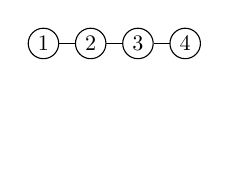
\begin{tikzpicture}[scale=0.6, every node/.style={scale=0.8,inner sep=.7mm}]
          \node [draw,circle] (1) at (0,0) {1};
          \node [draw,circle] (2) at (1,0) {2};
          \node [draw,circle] (3) at (2,0) {3};
          \node [draw,circle] (4) at (3,0) {4};
	  \node[] () at (0,-2.5) {};   % just to move the picture up a bit
          \draw (1) -- (2);
          \draw (2) -- (3);
          \draw (3) -- (4);
        \end{tikzpicture}
        \label{fig:assoc-g}
    }
    \quad\subfigure[][$H$] {
        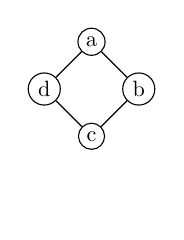
\begin{tikzpicture}[scale=0.6, every node/.style={scale=0.8,inner sep=.7mm}]
          \node [draw,circle] (a) at (1,2) {a};
          \node [draw,circle] (b) at (2,1) {b};
          \node [draw,circle] (c) at (1,0) {c};
          \node [draw,circle] (d) at (0,1) {d};
	  \node[] () at (0,-1.5) {};   % just to move the picture up a bit
          \draw (a) -- (b);
          \draw (b) -- (c);
          \draw (c) -- (d);
          \draw (d) -- (a);
        \end{tikzpicture}
        \label{fig:assoc-h}
    }
    \quad\subfigure[][Association graph] {
        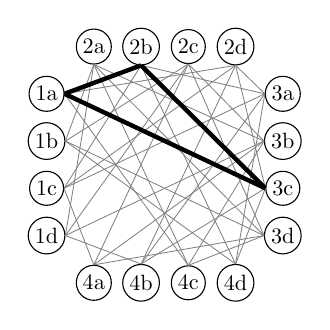
\begin{tikzpicture}[scale=0.6, every node/.style={scale=0.8,inner sep=.5mm}]
          \node [draw,circle] (1a) at (0,4) {1a};
          \node [draw,circle] (1b) at (0,3) {1b};
          \node [draw,circle] (1c) at (0,2) {1c};
          \node [draw,circle] (1d) at (0,1) {1d};
          \node [draw,circle] (2a) at (1,5) {2a};
          \node [draw,circle] (2b) at (2,5) {2b};
          \node [draw,circle] (2c) at (3,5) {2c};
          \node [draw,circle] (2d) at (4,5) {2d};
          \node [draw,circle] (3a) at (5,4) {3a};
          \node [draw,circle] (3b) at (5,3) {3b};
          \node [draw,circle] (3c) at (5,2) {3c};
          \node [draw,circle] (3d) at (5,1) {3d};
          \node [draw,circle] (4a) at (1,0) {4a};
          \node [draw,circle] (4b) at (2,0) {4b};
          \node [draw,circle] (4c) at (3,0) {4c};
          \node [draw,circle] (4d) at (4,0) {4d};
	  \draw[color=gray, line width=.3] (1a.east) -- (2d.south);
\draw[color=gray, line width=.3] (1a.east) -- (4c.north);
\draw[color=gray, line width=.3] (1b.east) -- (2a.south);
\draw[color=gray, line width=.3] (1b.east) -- (2c.south);
\draw[color=gray, line width=.3] (1b.east) -- (3d.west);
\draw[color=gray, line width=.3] (1b.east) -- (4d.north);
\draw[color=gray, line width=.3] (1c.east) -- (2b.south);
\draw[color=gray, line width=.3] (1c.east) -- (2d.south);
\draw[color=gray, line width=.3] (1c.east) -- (3a.west);
\draw[color=gray, line width=.3] (1c.east) -- (4a.north);
\draw[color=gray, line width=.3] (1d.east) -- (2a.south);
\draw[color=gray, line width=.3] (1d.east) -- (2c.south);
\draw[color=gray, line width=.3] (1d.east) -- (3b.west);
\draw[color=gray, line width=.3] (1d.east) -- (4b.north);
\draw[color=gray, line width=.3] (2a.south) -- (3b.west);
\draw[color=gray, line width=.3] (2a.south) -- (3d.west);
\draw[color=gray, line width=.3] (2a.south) -- (4c.north);
\draw[color=gray, line width=.3] (2b.south) -- (3a.west);
\draw[color=gray, line width=.3] (2b.south) -- (4d.north);
\draw[color=gray, line width=.3] (2c.south) -- (3b.west);
\draw[color=gray, line width=.3] (2c.south) -- (3d.west);
\draw[color=gray, line width=.3] (2c.south) -- (4a.north);
\draw[color=gray, line width=.3] (2d.south) -- (3a.west);
\draw[color=gray, line width=.3] (2d.south) -- (3c.west);
\draw[color=gray, line width=.3] (2d.south) -- (4b.north);
\draw[color=gray, line width=.3] (3a.west) -- (4b.north);
\draw[color=gray, line width=.3] (3a.west) -- (4d.north);
\draw[color=gray, line width=.3] (3b.west) -- (4a.north);
\draw[color=gray, line width=.3] (3b.west) -- (4c.north);
\draw[color=gray, line width=.3] (3c.west) -- (4b.north);
\draw[color=gray, line width=.3] (3c.west) -- (4d.north);
\draw[color=gray, line width=.3] (3d.west) -- (4a.north);
\draw[color=gray, line width=.3] (3d.west) -- (4c.north);
\draw[ultra thick] (1a.east) -- (2b.south);
\draw[ultra thick] (1a.east) -- (3c.west);
\draw[ultra thick] (2b.south) -- (3c.west);

        \end{tikzpicture}
        \label{fig:assoc}
    }
    \caption{Two graphs and their association graph.  The edges of a maximum
    clique in the association graph are highlighted. This corresponds to a maximum
    common induced subgraph: the subgraph of $G$ induced by $\{1,2,3\}$,
    which is isomorphic to the subgraph of $H$ induced by $\{a,b,c\}$.}
    \label{fig:intro-assoc-graph}
\end{figure}

A number of early algorithms for finding a maximum common subgraph use a \emph{maximal}
clique algorithm \citep{DBLP:journals/cacm/BronK73} for the maximisation problem
\citep{durand1999efficient,DBLP:conf/mco/VismaraV08}.

\citet{DBLP:conf/sspr/BunkeFGSV02} use the maximum clique algorithm of
\citet{DBLP:journals/siamcomp/BalasY86} to find a maximum common subgraph.
This algorithm greedily colours vertices during search to obtain a good upper
bound.  The RASCAL algorithm \citep{raymond2002rascal}---which solves MCES by
finding a maximum clique in the modular product graph of line graphs---tries
several other heuristic colouring methods in addition to greedy colouring, and
uses the one that gives the tightest upper bound.  Unfortunately the authors
were unable to provide code for RASCAL.

\cite{DBLP:conf/cp/McCreeshNPS16} use a state of the art maximum clique
algorithm, MCSa1
\citep{DBLP:journals/algorithms/Prosser12,DBLP:journals/ieicet/TomitaSHW13},
to solve the maximum common induced subgraph problem.  In addition to greedy
colouring, this algorithm uses a static vertex order based on degree, and has
very fast operations on sets due to the use of bitsets and the separate
compilation of code for different bitset sizes.  The paper also introduces a
modified version of the algorithm to solve the maximum common \emph{connected}
induced subgraph problem.

\subsection{Constraint Programming Algorithms}

\citet{DBLP:journals/spe/McGregor82}
introduced a branch and bound algorithm for the maximum common
\emph{edge} subgraph problem in which a vertex of $G$ is mapped to a vertex
of $H$ at each node of the search tree.  A matrix of Boolean values indicates
the set of edges in $H$ to which each edge in $G$ may be mapped; this may be
viewed as a simple domain store. \citet{DBLP:conf/sspr/BunkeFGSV02}
reports using McGregor's algorithm to solve MCIS, without giving full
details of the modifications made to the algorithm.

\citet{DBLP:conf/mco/VismaraV08} give a constraint model for solving maximum
common connected edge subgraph based on solving MCIS on the line graphs of the
two input graphs; effectively, this is the first formal constraint program for
MCIS.  Like the CP model for induced subgraph isomorphism in
\Cref{subsec:cp-model-isip}, we have a variable $x_v$ for each $v \in V(G)$.
Each domain is $V(H) \cup \bot$, where $\bot$ is a special value indicating that
a vertex is unmapped.  The objective is to minimise the number of $\bot$
values.  The model uses binary constraints to ensure that no two vertices in
$G$ are mapped to the same vertex in $H$.  The adjacency and non-adjacency
constraints from our induced subgraph isomorphism model are replaced by the
following, in order to allow any vertex to be mapped to $\bot$.

\begin{itemize}
    \item For all distinct $v, w \in V(G)$ such that $v \in N_G(w)$, we have 
$x_v=\bot$,
$x_w=\bot$, or
$x_v \in N_H(x_w)$.
\item For all distinct $v, w \in V(G)$ such that $v \not\in N_G(w)$, we have 
$x_v=\bot$,
$x_w=\bot$, or
$x_v \not\in N_H(x_w)$.
\end{itemize}

\citet{DBLP:conf/cp/NdiayeS11} present a CP model that shares the variables
of the \citeauthor{DBLP:conf/mco/VismaraV08} model, but replaces the binary difference
constraints with a single global ``soft allDiff''
constraint \citep{DBLP:conf/cp/PetitRB01}.  This ensures that distinct vertices
in $G$ are mapped to distinct vertices in $H$, and uses a matching algorithm
to calculate a stronger upper bound than the one given by
the \citeauthor{DBLP:conf/mco/VismaraV08} model.
\citeauthor{DBLP:conf/cp/NdiayeS11} carry out detailed experiments using
different levels of consistency for the adjacency and soft allDiff constraints.
The soft allDiff constraint, if it is used to calculate an upper bound but
not to filter domains, causes the algorithm to run several times faster
than the simple difference constraints used by \citeauthor{DBLP:conf/mco/VismaraV08}.
Comparing forward checking (FC) and maintaining arc consistency (MAC)
on the adjacency constraints, FC outperforms MAC on unlabelled instances
while MAC outperforms FC on labelled instances.

\cite{DBLP:conf/cp/McCreeshNPS16} add a connectedness constraint to the CP
model of \citet{DBLP:conf/cp/NdiayeS11}.  This is found to perform better
overall than ensuring connectedness simply by branching on vertices adjacent to
some already-mapped vertex.

Finally, the \kDown\ algorithm of \citet{UpcomingAAAIPaper}
solves the optimisation problem as a sequence of decision problems, with
each of these subproblems solved by a modified Glasgow algorithm
\citep{DBLP:conf/cp/McCreeshP15}.  It remains possible to filter
domains using supplemental graphs, albeit with weaker propagation
than for induced subgraph isomorphism.

\subsection{Subgraph Enumeration Algorithms}

Finally, we mention briefly a very different technique that has been used
in a number of papers to find a maximum common connected subgraph between two or more
graphs representing molecules
\citep{armitage1967automatic,takahashi1987recognition,DBLP:journals/jcheminf/DalkeH13}.
In this type of algorithm, connected
subgraphs of the first graph are enumerated by backtracking search.
A subgraph isomorphism solver is used to test whether each of these subgraphs
appears in each of the other input graphs.  In some versions of this algorithms,
the subgraphs of $G$ are tested for isomorphism with previously generated subgraphs
in order to break symmetries.
Unfortunately, we have been unable to find an implementation of this technique
for MCIS in general graphs to use in our experimental evaluation.

%% \subsection{Misc stuff to sort out}
%% 
%% \citet{cao2008maximum} is a backtracking algorithm that does not store domains,
%% but tests before making each assignment $(v,w)$ whether the set of vertices in $M$
%% that are adjacent to $v$ in $G$ corresponds to the set of vertices in $M$ that
%% are adjacent to $w$ in $H$.  The main upper bound proposed by the authors
%% is, in CP terms, the bound given by adding to $|M|$ the number of unassigned
%% variables whose domains contain at least one vertex.  The authors also outline
%% a matching upper bound.  In each case, it appears likely that the fact that the algorithm does not
%% store domains results in substantial addition work on each call of the upper bound
%% function.  (TODO tidy up that last sentence!)

%% \section{New algorithms in this thesis}
%% 
%% The McSplit family of algorithms has branch-and-bound variants and variants
%% that use a sequence of decision problems; it also has variants for induced and
%% edge subgraph problems. The summary in this section discusses only the induced
%% variants.
%% 
%% McSplit performs tree search in the style of a forward-checking constraint
%% programming algorithm. Rather than maintaining an explicit domain for each
%% vertex in the first graph, vertices are re-labelled at each search node in such
%% a way that the current mapping may only be extended by mapping a vertex in
%% first graph to a vertex in the second graph with the same label. Labels may be
%% viewed as equivalence classes of vertices, and at each search node these
%% classes are refined (partitioned) into smaller classes. We store the vertices
%% of each graph as a list (without copying at each search node), and can perform
%% this partitioning efficiently be re-arranging the vertices in each list. This
%% data structure makes it possible to calculate an upper bound very cheaply at
%% each search node, and permits the cheap computation of good variable-ordering
%% heuristics.

\section{Experimental details}\label{sec:experimental-details}

\subsection{Experimental setup}

The primary experimental setup used for this dissertation was a cluster
of machines with dual Intel Xeon E5-2697A v4 CPUs with thermal scaling disabled
and 512GBytes RAM. All code was compiled with GCC version 9.4.0.
All algorithms used are sequential; 32 instances
(one per CPU core) were solved concurrently.
This setup was used except where indicated otherwise: namely, in
\Cref{sec:mcsplit-experiments} and \Cref{c:universal-graphs}.

All of the new algorithms presented were implemented by the present author in
C++ (Chapters \ref{c:mcsplit-i-undirected} to \ref{c:mcsplit-si})
and Python (Chapter \ref{c:universal-graphs}).  All solvers by other
authors were implemented either in C or C++.  Throughout, the 
compiler flag \texttt{-O3} (optimization level 3) was used.

\subsection{Conventions for Plots}

Scatter plots and cumulative plots are used frequently in this dissertation to
compare the run times of algorithms.  To illustrate how these will be used,
consider the run times in milliseconds for ten hypothetical instances,
with one row per instance, in \Cref{fig:intro-dummy-table}.

\Cref{fig:intro-dummy-scatter} shows a scatter plot of these run times. Log
scales are used for run times throughout this dissertation. Since run times are
measured at a 1 millisecond resolution, the points are jittered by adding a
uniform random number in the range $[-1/2,1/2)$ to each time. This reduces
over-plotting and thus helps to show the distribution of points, with only a
negligible effect on the plots' precision. Run times of zero are plotted in the
range $[1/2,1)$ because zero cannot appear on a log scale.  Timeouts (exceeding
1000 seconds) appear in the grey band just beyond a run time of 1000 seconds;
again, we jitter these within the band to minimise over-plotting. The line
$x=y$, where the two algorithms have the same run time, is show for
convenience.

\Cref{fig:intro-dummy-cumu} shows a less common type of figure: an
\emph{empirical cumulative distribution function plot} (henceforth
\emph{cumulative plot}). For a given run time $t$ (on the horizontal axis),
this answers the question ``how many of the instances can be solved in less
than $t$ milliseconds per instance?'' Equivalently, it answers the question
``if the per-instance time limit were reduced to $t$, how many instances would
each algorithm solve?''
We can see, for example, that Algorithm A can solve six
of the instances within 10 ms (the first six instances in the table),
while Algorithm B can solve only three instances
within that time.

\begin{figure}[htb]
    \centering
    \subfigure[][Hypothetical run times per instance] {
        \tiny
        \includegraphics*[width=0.2\textwidth]{10-introduction/plot-examples/table/table}
        \label{fig:intro-dummy-table}
    }
    \subfigure[][Scatter plot of run times] {
        \includegraphics*[width=0.39\textwidth]{10-introduction/plot-examples/plots/scatter}
        \label{fig:intro-dummy-scatter}
    }
    \subfigure[][Cumulative plot of run times] {
        \includegraphics*[width=0.34\textwidth]{10-introduction/plot-examples/plots/cumulative}
        \label{fig:intro-dummy-cumu}
    }
    \caption{Hypothetical run times in ms for two solvers on ten instances: table,
        scatter plot, and cumulative plot. The time limit is 1000 seconds.}
    \label{fig:intro-dummy-figs}
\end{figure}

%\section{Miscellaneous notes}
%
%MCIS is \NP-hard, even if graphs are both bipartite.  This can be shown by a
%reduction from maximum induced matching.  (I think the proof for maximum induced
%matchings is in Induced Matchings (1989) by Kathie Cameron). Is there another
%proof somewhere? David: Yes, see http://dx.doi.org/doi:10.1016/j.jda.2004.05.001 for a survey of the early results
%
%See David's notes - something about Stockmeyer and Vazirani 1982 NP-completeness of some ... ?
%
%Independent set is NP-hard on planar graphs (see Wikipedia).  Therefore
%MCIS also is.
%
%Cuissart and Hebrard 2005 A Direct Algorithm to Find a Largest Common
%Connected Induced Subgraph of Two Graphs doesn't seem to do any
%pruning.  Is it slow?
%
